\documentclass[a4paper,11pt]{article}

\usepackage[utf8]{inputenc}
\usepackage[italian]{babel}
\usepackage{graphicx}
\usepackage{geometry}

\newgeometry{vmargin={10mm,28mm}, hmargin={25mm,25mm}}

% Definition of \maketitle
\makeatletter
\newcommand{\departmentname}[1]{\def\@departmentname{#1}}
\newcommand{\coursename}[1]{\def\@coursename{#1}}
\newcommand{\academicyear}[1]{\def\@academicyear{#1}}
\newcommand{\advisorname}[1]{\def\@advisorname{#1}}
\newcommand{\coadvisorname}[1]{\def\@coadvisorname{#1}}
\newcommand{\studentname}[1]{\def\@studentname{#1}}
\newcommand{\itathesistitle}[1]{\def\@itathesistitle{#1}}
\newcommand{\engthesistitle}[1]{\def\@engthesistitle{#1}}

\def\@maketitle{
	\begin{center}
		
\includegraphics[width=4cm]{images/logoUnipr.png}\\[2ex]
		\@departmentname\\[1ex]
		\@coursename\\
		\noindent\rule{8cm}{0.4pt}\\[1ex]
		\@itathesistitle\\[1ex]
		\@engthesistitle
	\end{center}
	\underline{Relatore:}
	\hfill
	\underline{Tesi di Laurea di:}\\
	\@advisorname
	\hfill
	\@studentname\\[1ex]
	\underline{Correlatore:}\\
	\@coadvisorname
	\begin{center}
		\@academicyear
	\end{center}
	\vskip 0.1cm
}
\makeatother

\departmentname{\textbf{Dipartimento di Ingegneria e Architettura}}
\coursename{\textbf{Corso di Laurea in Ingegneria Informatica Elettronica e delle Telecomunicazioni}}
\academicyear{ANNO ACCADEMICO 2020/2021}
\advisorname{Chiar.mo Prof. Michele Amoretti}
\coadvisorname{Dott. Ing. Gabriele Penzotti}
\studentname{Filippo Scaramuzza}
\itathesistitle{Simulazione di Sistemi Fog N-Tier con Posizionamento Dinamico dei Servizi}
\engthesistitle{Simulation of N-Tier Fog Systems with Dynamic Service Placement}

\begin{document}
	\maketitle

Nell'era dei Big Data il tempo richiesto per accedere ad alcune applicazioni \textit{Cloud-based}, che concentrano l'intera elaborazione dei dati nei \textit{data center}, potrebbe essere troppo elevato. Inoltre, l'ormai noto incremento dei dispositivi connessi in ambito Internet of Things, ed il conseguente rapido aumento dei dati generati nell'edge della rete richiedono l'implementazione del cosiddetto \textit{Cloud-to-Thing Continuum}. In questo ambito sono state avanzate numerose proposte, ad esempio il \textit{Fog Computing}, un paradigma a livello di sistema che distribuisce le funzioni di elaborazione, archiviazione, controllo e comunicazione dall'edge al Cloud. I possibili ambiti di applicazione del \textit{Fog Computing} sono innumerevoli: dagli \textit{Smart Vehicles} al \textit{Traffic Control}, alle \textit{Smart Cities} e agli \textit{Smart Buildings}.

Questo lavoro di Tesi nasce da un periodo di Internato di Laboratorio presso il Dipartimento di Ingegneria e Architettura dell'Università di Parma, il cui obiettivo è stato quello di realizzare simulazioni di sistemi Fog, con lo scopo di poter analizzare questo paradigma in un'architettura \textit{N-Tier}, implementando anche uno specifico algoritmo di placement dei servizi.

L'architettura di riferimento ha una struttura composta da 3 macro-entità: il Cloud, il livello Fog e gli end-node/dispositivi IoT. Il livello Fog, inoltre, è ulteriormente scomposto in sotto-livelli (tier) che più sono distanti dai dispositivi, più aumentano le loro capacità computazionali.

\begin{figure}[!ht]
  \includegraphics[width=8cm]{images/FogCloudToThingContinuum}
  \centering
  \caption[Architettura OpenFog N-Tier]{Architettura OpenFog N-Tier.}
  \label{fig:ntier_architecture}
\end{figure}

Il software realizzato si basa su \textit{YAFS} (\textit{Yet Another Fog Simulator}), un simulatore ad eventi discreti sviluppato in Python ed a sua volta basato su \textit{SimPy}, ovvero un framework DES (\textit{Discrete Event Simulator}) basato sui processi, anch'esso sviluppato in Python.

Nel \textit{Capitolo 1} vengono introdotti i principali concetti fondanti del \textit{Cloud Computing}, del \textit{Fog Computing} e degli altri principali paradigmi in quest'ambito di ricerca. Vengono poi citate possibili applicazioni del \textit{Fog Computing} e viene fatta una breve introduzione a YAFS. Nel \textit{Capitolo 2} vengono affrontati i dettagli implementativi del simulatore YAFS, la sua struttura e la modellazione delle simulazioni. Successivamente vengono approfondite le caratteristiche degli scenari simulati in questo lavoro di Tesi. Nel \textit{Capitolo 3} vengono trattati i principali aspetti del sistema di simulazione realizzato. Vengono poi discusse le modalità di utilizzo e le analisi che si possono eseguire. Nel \textit{Capitolo 4}, vengono presentati i principali risultati ottenuti dalle simulazioni eseguite. Vengono in particolare valutati l'algoritmo di placement utilizzato al variare di specifici parametri di configurazione del sistema ed il soddisfacimento delle richieste con e senza failure control. In conclusione, vengono discussi il lavoro svolto e i possibili sviluppi futuri.

Lo strumento sviluppato si è dimostrato piuttosto flessibile, permettendo la valutazione dei diversi aspetti architetturali e di configurazione dei sistemi Fog. Il Fog Computing è caratterizzato da un approccio distribuito, derivante dal bisogno di superare i limiti dell'approccio centralizzato del Cloud Computing. Infatti i nodi Fog possono essere posizionati ovunque nella rete tra gli end-node e il Cloud. Questa flessibilità apre molti interrogativi che possono essere fugati tramite software di simulazione come quello realizzato. 

\begin{figure}[!ht]
  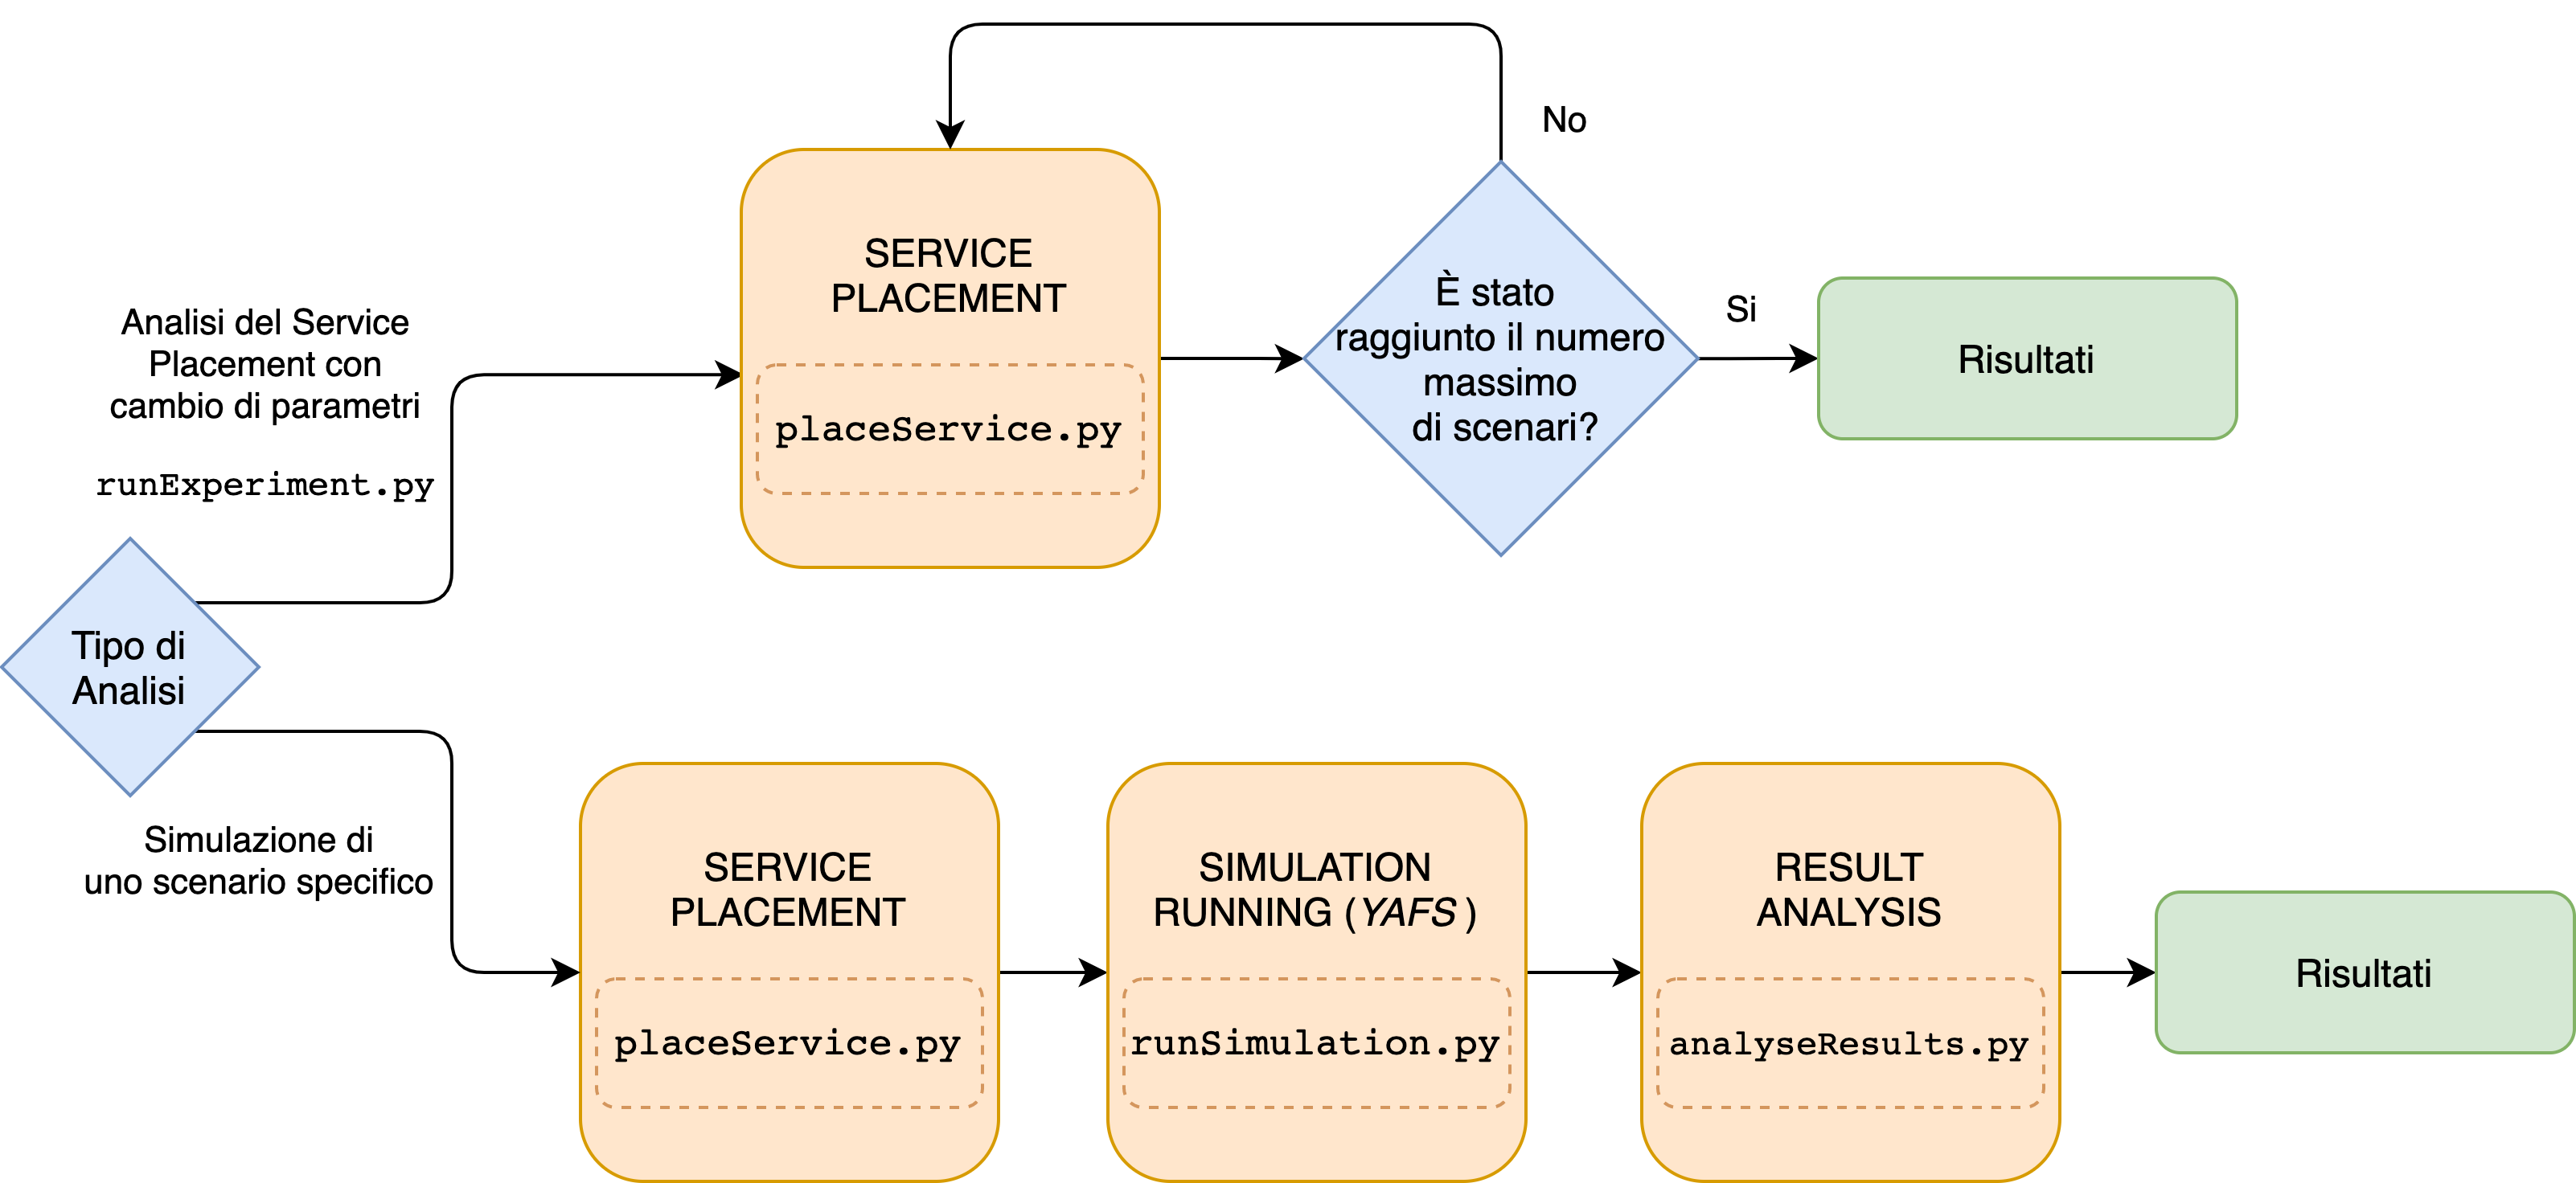
\includegraphics[width=10cm]{images/sim_flow_diagram}
  \centering
  \caption{Diagramma di flusso del sistema di simulazione.}
  \label{fig:sim_flow_diagram}
\end{figure}

Sono stati ottenuti diversi risultati rilevanti, come l'andamento del successo dell'algoritmo di placement dei servizi al variare della distribuzione della privacy, delle risorse richieste dai servizi, dell'interconnessione tra i nodi a livello Fog, del numero di questi nodi, e del numero di servizi per ogni applicazione. Questo ha permesso di chiarire quali sono i parametri che più influenzano il successo dell'algoritmo, anche valutando le prestazioni durante la simulazione di un sistema così configurato.

Nella fase di Internato di Laboratorio è stato fatto un lavoro di ricerca sugli aspetti trattati nel Capitolo 1 e che sono serviti per la definizione delle simulazioni, della topologia di rete e per l'analisi dei risultati. Il software realizzato, però, si presta a diverse tipologie di analisi: si può pensare ad un'implementazione di un'architettura differente, di un diverso algoritmo di placement, o a diversi tipi di applicazioni che possono essere allocate nella rete. 

L'IoT ha accelerato la cosiddetta ``trasformazione digitale" e fornisce benefici sia ai singoli utenti che alle aziende di diversi settori, come energia, trasporti, istruzione, sanità pubblica e così via. Proprio grazie all'IoT, il numero di dispositivi connessi è in forte crescita e con questo anche la quantità di dati che vengono prodotti.

Il Fog Computing, unitamente alle sue principali estensioni esposte nel Capitolo 1, si offre come una delle soluzioni più promettenti per la gestione dei Big Data che vengono prodotti dai dispositivi IoT.


   	\end{document}